\documentclass[10pt,a4paper]{article}
\usepackage[utf8]{inputenc}
\usepackage[spanish]{babel}
\usepackage{amsmath}
\usepackage{amsfonts}
\usepackage{amssymb}
\usepackage{graphicx}
\usepackage{multicol}
\usepackage{titling}
\usepackage{titlesec}
\usepackage{array}
\usepackage{bm}
\usepackage{afterpage}
\usepackage{booktabs} %LIBRERIA PARA EXCE
\usepackage{multirow}
\usepackage{float}
\usepackage{pdfpages}
\usepackage{graphicx}
\usepackage{epstopdf}
\usepackage{longtable}
\usepackage{xcolor}
\usepackage{color}
\usepackage{epigraph}
\setlength\epigraphwidth{1.5\textwidth}
\usepackage{subfigure}
\usepackage{anyfontsize}
\usepackage[left=2cm,right=2cm,top=2cm,bottom=2cm]{geometry}
\usepackage[colorlinks=true,
            linkcolor=blue,
            citecolor=blue,
            urlcolor=blue]{hyperref}

\begin{document}
\author{Cauja María José, Chandi Armando, Nazate Marisol, Valencia Fernando} % CAMBIAR A AUTORES
\title{\textbf{SISTEMAS DE MEDICIÓN DE CALIDAD DEL AIRE}}
\date{13 de diciembre de 2019}
\maketitle  

\section{Introdución}


Actualmente la polución ambiental es uno de los principales problemas a nivel mundial. Debido a las altas concentraciones de contaminación atmosférica se presentan efectos negativos para la ciudadanía, ya que a causa de los contaminantes nocivos se registra una mayor tasa de enfermedades y problemas respiratorios. En consecuencia se presentan efectos económicos considerables, ya que acorta la vida, aumenta los costes médicos y reduce la productividad. Por lo tanto es necesario usar un medidor de calidad del aire, pues de esa manera se puede tomar las precauciones necesarias para evitar ese tipo de problemas o al menos reducir en gran parte los efectos negativos.

\section{Resumen}

Hoy en día el problema de la contaminación ambiental ha ido en crecimiento, por lo cual causa grandes pérdidas  a nivel mundial, tanto a nivel social, económico y de salud, por lo que se ha visto la necesidad de realizar la implementación de un sistema que pueda medir la calidad del aire. El principal objetivo es realizar un análisis de la calidad del aire en varios puntos de muestreo más considerables y representativos para la obtención de datos reales, útiles y que presenten margen de error en cantidades mínimas. Uno de los principales métodos de solución que contribuyen a la calidad del aire y efectos sobre la salud son las redes inalámbricas de sensores. A continuación se realizará un breve análisis de algunos de los sistemas que se pueden utilizar. Actualmente se utilizan varios sensores para supervisión de agentes contaminantes en el aire con el fin de determinar el grado de pureza de oxígeno y como este influye en una población específica, un ejemplo son los sensores de quimioluminiscencia los cuales ejecutan un principio de medición que se basa en la reacción radioactiva del ozono con óxido de nitrógeno (NO) permitiendo medir su cantidad, otro agente externo es el NOx (x puede ser cualquier valor) el cual se puede medir mediante la separación de NO por la luz UV (ultravioleta). Por otro lado se tiene el impacto de la emisión de NOx en el clima y el monitoreo utilizando tecnología de sensores inteligentes Este es un sistema que se plantea para desarrollar un clasificador inteligente de monitorización y control de la calidad de combustión de temperatura y NOx. El principal objetivo es la detección, el reconocimiento y comprensión de las condiciones de combustión mediante la utilización de sensores inteligentes, los cuales son operados y controlados por un sistema basado en análisis de datos con un límite umbral. Otro de los sistemas propuesto es el llamado Pulluino, el cual corresponde a una gestión eficiente basada en la nube de dispositivos IoT para monitoreo de calidad del aire Es un sistema que sirve para el control de la contaminación del aire, mediante una eficiente nube basada en gestión de dispositivos IO para el monitoreo del aire. Estos dispositivos inteligentes son capaces de detectar, almacenar y analizar los flujos de datos en una red de información y comunicación. Dentro de los diversos sistemas se tiene también el desarrollo de plataforma de detección para mediciones y análisis de calidad del aire para obtener datos acerca de la calidad del aire a partir de un ensamblaje de bajo costo en Arduino el cual muestra los datos de una forma simple en una pantalla LCD así mismo permite visualizar índices de contaminación en función a la combinación de luces LED, este sistema capturó datos de SPM (partículas suspendidas), NRMF (el respirable de las partículas suspendidas), SO2, etc; los cuales pueden ser utilizados para un posterior estimaciones de contaminación a la que están expuestos los seres vivos. Finalmente se tiene el sistema de monitoreo de contaminación de aire urbano con modelos de predicción debido a que este sistema utiliza sensores gaseosos y meteorológicos que realizan el monitoreo del nivel de contaminación en el aire de una zona urbana determinada, los datos adquiridos se envían a una base de datos la cual procesaría y mostraría únicamente los datos que puedan servir como información útil para una posterior predicción del nivel de contaminación. Todos estos sistemas son indicados para determinar la detección de posibles malas condiciones ambientales, pues es de gran relevancia debido a que es capaz de contribuir a varios campos de aplicación y sectores del mercado especialmente para mejorar las condiciones medioambientales y por ende la calidad de vida. 

\section{Diseño del sistema}
\subsection{Placa del sistema}

Para el desarrollo del siguiente proyecto se usará una placa de desarrollo MCU, en conjunto con Arduino Uno como se muestra en la Figura 1., los cuales nos permitirá realizar las conexiones de los diferentes sensores


\begin{figure}[H]
\centering
 \includegraphics[scale=0.8]{NodeMCU.JPG} 
 \includegraphics[scale=0.4]{arduino.JPG} 
\caption{NodeMCU Tercera Generación v3  /  Arduino} 
\end{figure}

Se ensamblará los diferentes sensores en una baquelita, diseñando así las pistas de las conexiones que corresponden para cada uno de los dispositivos

\subsection{Conexiones}

Se debe tener en cuenta un diseño de conexiones de todos los dispositivos para el funcionamiento del sistema, se crea en el software libre Fritzing siendo un programa que nos permite hacer esquemas eléctricos, y diseñar nuestro PCB final.

\begin{figure}[H]
\centering
 \includegraphics[scale=0.80]{Fritzing.JPG} 
\caption{Diseño en Fritzing} 
\end{figure}

Las conexiones que se realizan constan de: tres leds con sus respectivas resistencias los cuales nos permitirá revelar los diferentes parámetros, y los diferentes enlaces de los sensores NodeMCU, DHT11, MQ-135, y Sensor Rayo UV GYM L8511

\subsection{Diagrama de conexión }

Para la realización del diagrama de pistas en la PCB, se lo ejecuto en el software PCB Wizard, siendo aquel que permite crear esquemas de circuitos electrónicos y a partir de estos, obtener de una manera sencilla el diseño del circuito impreso a una o dos caras

\begin{figure}[H]
\centering
 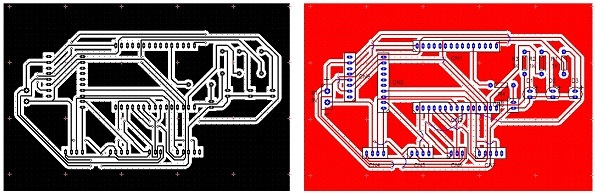
\includegraphics[scale=0.68]{placasensores.JPG} 
\caption{Pista esquemática PCB} 
\end{figure}

El proceso de fabricación de una placa PCB, se lo realizo con una impresión laser del circuito en papel couche, luego se lo recorta el circuito del tamaño necesario que necesita la lámina circuital, para consiguiente planchar el recorte sobre la baquelita de cobre, siendo que la tinta a laser y el papel couche, se quede impregnada en la placa por el calor; finalmente a la baquelita se lo pone en acido por unos minutos, y por siguiente el cobre sobrante se eliminando, quedando así las pistas conductoras de cobre. 
A continuación de este proceso se realizan las perforaciones con taladro de broca delgada, teniendo cuidado que las pistas puedan ser afectadas.\\

\begin{figure}[H]
\centering
 \includegraphics[scale=0.80]{disefrontal.JPG} 
\caption{Diagrama - PCB} 
\end{figure}

El proceso de fabricación de una placa PCB, se lo realizo con una impresión laser del circuito en papel couche, luego se lo recorta el circuito del tamaño necesario que necesita la lámina circuital, para consiguiente planchar el recorte sobre la baquelita de cobre, siendo que la tinta a laser y el papel couche, se quede impregnada en la placa por el calor; finalmente a la baquelita se lo pone en acido por unos minutos, y por siguiente el cobre sobrante se eliminando, quedando así las pistas conductoras de cobre. 
A continuación de este proceso se realizan las perforaciones con taladro de broca delgada, teniendo cuidado que las pistas puedan ser afectadas\\


\section{Desarrollo}

\subsection{Diagrama de Bloques}

\begin{figure}[H]
\centering
 \includegraphics[scale=0.90]{bloquecito.JPG} 
\caption{Proceso del Sistema } 
\end{figure}

\subsection{Diagrama de Flujo}

\begin{figure}[H]
\centering
 \includegraphics[scale=0.95]{flujos.JPG} 
\caption{Procedimiento para obtención de datos } 
\end{figure}


\subsection{Selección de los sensores}

Para poder escoger entre estos sensores se procedió a comparar con varios tipos; existen diferentes opciones tanto genéricas como profesionales para efectos del proyecto serán necesarios sensores que puedan obtener datos de aire, humedad y temperatura.\\\\

\textbf{Placa NodeMCU}\\

Es de código abierto basado en el chip ESP8266 (ESP-12E), que utiliza el lenguaje de programación Lua para crear un ambiente de desarrollo para aplicaciones que requiera conectividad Wifi de manera rápida.
El ESP8266 ofrece una solución completa y autónoma de redes Wi-Fi, lo que le permite alojar la aplicación o servir como puente entre Internet y un microcontrolador, tiene potentes capacidades a bordo de procesamiento y almacenamiento que le permiten integrarse con sensores y dispositivos específicos de aplicación.\\\\

\textbf{Sensor DHT-11}\\

El DHT11 es un sensor de humedad relativa y temperatura de bajo costo y de media precisión. Integra un sensor capacitivo de humedad y un termistor para medir el aire circundante, y muestra los datos mediante una señal digital en el pin de datos . \\\\\\\\\\

\textbf{Sensor MQ-7}\\

Este sensor es de alta sensibilidad al monóxido de carbono (CO), pero también es sensible al H2.  Puede detectar concentraciones en el rango de 20 a 2000ppm.
El módulo posee una salida analógica que proviene del divisor de voltaje que forma el sensor y una resistencia de carga. También tiene una salida digital que se calibra con un potenciómetro, esta salida tiene un led indicador.\\\\

\textbf{Sensor MQ-135}\\

Se utilizan en equipos de control de calidad del aire para edificios y oficinas, son adecuados para la detección de NH3, NOx, alcohol, benceno, humo, CO2, etc
Este sensor no proporciona valores absolutos, sino que simplemente proporciona una salida analógica que debe ser monitoreado y se comparada con los valores de umbral.\\\\

\textbf{Sensor Rayos UV GYML8511}\\

Este sensor UV, se utiliza para detectar el índice de intensidad ultravioleta (UV). Tiene una amplia gama espectral de 200nm hasta 370nm*. La señal eléctrica de salida del módulo, es de tipo analógica, que varía respecto a la intensidad de los rayos.\\\\

\textbf{Multiplexor 74HC4051}\\

Proporciona acceso a todos los pines y características del 74HC4051, un multiplexor/ demultiplexor analógico de 8 canales. El 74HC4051 le permite convertir cuatro pines de E/S en ocho señales multifuncionales, seleccionables individualmente, que se pueden utilizar para hacer de todo, desde controlar ocho LED hasta monitorear ocho potenciómetros.


\section{Tabla de datos}

\begin{figure}[H]
\centering
 \includegraphics[scale=0.80]{tabladatos.JPG} 
\caption{Valores de sensores en rangos de medida y valores obtenidos} 
\end{figure}

\begin{figure}[H]
\centering
 \includegraphics[scale=0.80]{tablamux.JPG} 
\caption{Pines del Multiplexor} 
\end{figure}


\section{PCB Wizard}

Es un software para la creación de placas de circuito impreso muy intuitivo y fácil de usar. PCB Wizard cuenta con muchas opciones que nos facilitarán el trabajo, como ser: generación de reportes, creación de archivos NC Drill y Gerber y múltiples opciones de impresión, entre otras. Si bien cuenta con las librerías y encapsulados más comunes puede que este sea el punto flojo del software. Igualmente no nos debemos preocupar demasiado ya que podemos crear nuestros propios componentes y guardarlos como librerías para su utilización en otro momento. 

\section{Algoritmos para suavizar señales}
\subsection{Mediana}

El filtro de mediana define una ventana de N elementos, que recoge las últimas N mediciones. El valor del filtro es la mediana de los valores contenidos en la ventana.
Aumentar el tamaño de la ventana aumenta el suavizado de la señal pero añade un retraso a la señal ya que es necesario "esperar" al muestreo de más puntos, se prefieren tamaños de ventana impares para evitar tener que promediar entre dos muestras, lo cual eliminaría parte de la capacidad de filtrado de la mediana. Siendo su formula:

\begin{equation}
z_{j}=median (x_{j-n}..x_{j-2},x_{j-1},x_{j},x_{j+1},x_{j+2}...x_{j+n})
\end{equation}

Para encontrar la mediana, las muestras de la ventana N-muestras se ordenan y la mediana se determina como:

\begin{equation}
\begin{Bmatrix}
S_{(n+1)/2} , & if  & N & mod 2==1 & \\
S_{N/2-1}+S_{N/2+1}, & if  &  N &  mod 2==1 & 
\end{Bmatrix}
\end{equation}

La fórmula describe la selección de la mediana de la lista ordenada S. si N es impar, la mediana es la muestra 
\begin{equation}
 S_{(n+1)/2} 
\end{equation}
 entonces la mediana es el promedio de dos elementos 
\begin{equation}
S_{N/2-1}  
 \end{equation} 
\begin{equation}
S_{N/2+1}
 \end{equation} 

\subsection{ Kalman}

El filtro de Kalman es un algoritmo que se basa en el modelo de espacio de estados de un sistema para estimar el estado futuro y la salida futura realizando un filtrado optimo a la señal de salida, y dependiendo del retraso de las muestras que se le ingresan puede cumplir la función de estimador de parámetros o únicamente de filtro. Pero en ambos casos elimina ruido, estas ecuaciones son ampliamente utilizadas ya que incluyen probabilidades estadísticas puesto que toma en cuenta la aleatoriedad tanto de la señal como del ruido. A diferencia de otros tipos de filtros este no requiere de una frecuencia de corte específica debido a que se basa en la característica del ruido permitiendo de esta manera filtrar en todo el espectro de frecuencias. Además sus ecuaciones solo dependen de una muestra anterior y la muestra presente lo que permite un ahorro considerable de memoria a la hora de ser implementado en un sistema digital y su fácil programación lo hace muy atractivo ya que se basa en un método recursivo.
Normalmente, el algoritmo requiere un cálculo de dos pasos procedimiento: paso de actualización de tiempo, llamado predicción y paso de actualización de medición, llamado corrección. Predicción da el estado actual estimado por adelantado y el la corrección ajusta la estimación proyectada usando la corriente medición. En el paso de predicción, la estimación del estado es calculado a partir de la siguiente ecuación:

\begin{equation}
\widehat{x} _{k}^{-} A.\widehat{x}_{_{k-1}}+B.\upsilon _{k-1}
\end{equation}

En el siguiente etapa del paso de predicción, el cálculo del error
Se debe realizar una proyección de covarianza. Su fórmula tiene la siguiente forma:

\begin{equation}
P_{k}^{-} A.P_{k-1}.A^{T}+Q
\end{equation}

La ganancia controla la influencia de la medición en la estimación del estado a posteriori en el paso de tiempo k. La ganancia de Kalman se calcula utilizando la siguiente fórmula:

\begin{equation}
K_{k}=P_{k}^{-}.H^{T}.(H.P_{k}^{-}+R)^{-1}
\end{equation}

El matriz R es la imprecisión de la medición (covarianza de ruido).  Finalmente, la fórmula para la actualización de estimación de estado con las medidas tiene la siguiente forma:

\begin{equation}
\widehat{x}_{k} = \widehat{x} _{k}^{-} + K_{k}.(zk-H.\widehat{x}_{k}^{-})
\end{equation}

Al final del procedimiento de actualización, la covarianza de error
Se requiere actualización. Su fórmula tiene la siguiente forma:

\begin{equation}
P_{k}=(I-K_{k}.H).P_{k}^{-}
\end{equation}


\subsection{Estimación de densidad de Kernel }

La estimación de densidad de kernel (KDE) es uno de los métodos no paramétricos que mejora algunas características estructurales en los datos no disponibles en el enfoque paramétrico. El estimador del núcleo f(x) estima la distribución de la densidad de probabilidad f de la señal. su fórmula tiene la siguiente forma:

\begin{equation}
\widehat{f}(x)= \frac{1}{mh^{n}}\sum_{i=1}^{m} K(\frac{x-x_{i}}{h})
\end{equation}

Donde h es el ancho de banda que controla la suavidad de la estimación, m el número de muestras, n las dimensiones del vector de señal X, señal unidimensional, entonces n = 1. K se llama el núcleo. Existen varias formas de núcleos y la selección del más apropiado se realiza típicamente sobre la base de un cálculo de error cuadrático medio integrado MISE (f). El núcleo uniforme no óptimo más simple tiene la siguiente forma:

\begin{equation}
K(\upsilon )=\begin{Bmatrix}
\frac{1}{2}, if \left | \upsilon  \right | \leq 1 & \\ 
0, if \left | \upsilon  \right | > 1 & 
\end{Bmatrix}
\end{equation}


\section{Diseño de Placa y Pruebas de funcionamiento}
\subsection{Diseño de Placa}


\begin{figure}[H]
\centering
 \includegraphics[scale=0.65]{creacion.JPG} 
\caption{Creación de placa mediante PCB Wizard}
\end{figure}

\begin{figure}[H]
\centering
\includegraphics[scale=0.65]{implementacion.JPG} 
\caption{Implementación de elementos electrónicos en la placa PCB} 
\end{figure}

\begin{figure}[H]
\centering
\includegraphics[scale=0.65]{circuito.JPG}
 \caption{Circuito medidor calidad de aire en placa PCB} 
\end{figure} 

\section{Resultados}
\subsection{Filtro Mediana}
En los resultados presentes como se puede apreciar en la primera figura se mostrará el filtro del sensor MQ7, se ve que se ha quitado la mayoría de los picos de la señal, lo que se corresponde para la eliminación de espurios y ruido, también se visualiza que existe un pequeño retardo con respecto a la señal original de igual forma en el sensor MQ135 y UV GYML8511.
Para el sensor MQ135 siendo este el que detecta los gases CO y CO2, el suavizado de la señal es mas visible ya que los datos extraídos tienen más variación de mínimos y máximos con relación al sensor anterior, mientras que para el sensor UV GYML8511, al tener una escala de normalidad entre 0-15 el filtrado en este caso al contener datos de magnitudes muy pequeñas pues la señal será casi nula, y se podrá visualizar en los picos más altos. El suavizado es producir cambios lentos en el valor para que sea más fácil ver las tendencias en nuestros datos.\\

Señal de datos de entrada 
Sensor: MQ7  Datos de muestra: 449 datos de variación de CO
Interpretación:  Línea azul – Datos, Línea roja- señal suavizada 

\begin{figure}[H]
\centering
\includegraphics[scale=0.65]{mediana1.JPG}
 \caption{Filtro mediano para sensor MQ7} 
\end{figure} 

Señal de datos de entrada 
Sensor: MQ135  Datos de muestra: 449 datos de variación de CO2
Interpretación:  Línea azul – Datos, Línea roja- señal suavizada 

\begin{figure}[H]
\centering
\includegraphics[scale=0.65]{mediana2.JPG}
 \caption{Filtro mediano para sensor MQ135} 
\end{figure} 

Señal de datos de entrada 
Sensor: UV GYML8511 		
Datos de muestra: 449 datos de variación de concentración de rayos UV es escala 0-15
Interpretación: Línea azul – Datos, Línea roja- señal suavizada 

\begin{figure}[H]
\centering
\includegraphics[scale=0.65]{mediana3.JPG}
 \caption{Filtro mediano para sensor UV} 
\end{figure} 

\subsection{Filtro Kalman}

En los gráficos que se presenta a continuación, se logra observar la señal de datos de muestra obtenidos por los sensores: MQ7, MQ135 y  UV GYML8511 con 449 datos de variación cada uno, los cuales son valores necesarios para poder lograr visualizar de mejor manera las gráficas de variación de CO, CO2 y Rayos UV respectivamente. Por otra parte, se tiene la señal suavizada que viene a ser el resultado de aplicar el filtro de Kalman, que en definitiva se trata de un algoritmo que se basa en un modelo de espacio de estados, es decir que relaciona la señal anterior con la señal presente, de tal manera que se pueda eliminar el ruido para obtener un  filtrado óptimo de la señal de salida, de acuerdo a los parámetros establecidos. \\

Señal de datos de entrada 
Sensor: MQ7  Datos de muestra: 449 datos de variación de CO
Interpretación: Línea azul – Datos, Línea roja- señal suavizada 

\begin{figure}[H]
\centering
\includegraphics[scale=0.65]{suave1.JPG}
 \caption{Señal de Datos y Señal Suavizada del sensor MQ7} 
\end{figure} 


Señal de datos de entrada 
Sensor: MQ135   Datos de muestra: 449 datos de variación de CO2
Interpretación:  Línea azul – Datos, Línea roja- señal suavizada 

\begin{figure}[H]
\centering
\includegraphics[scale=0.65]{suave2.JPG}
 \caption{Señal de Datos y Señal Suavizada del sensor MQ135} 
\end{figure} 

Señal de datos de entrada 
Sensor:  UV GYML8511 		
Datos de muestra:  449 datos de variación de concentración de rayos UV es escala 0-15
Interpretación: Línea azul – Datos, Línea roja- señal suavizada 
Al no realizar la toma de datos en tiempo real, la potencia es baja, hasta que se consiga la estabilización de la señal en aproximadamente 10 muestras más. 

\begin{figure}[H]
\centering
\includegraphics[scale=0.65]{suave3.JPG}
 \caption{Señal de Datos y Señal Suavizada del sensor UV GYML8511} 
\end{figure} 

\subsection{Filtro Kernel}


\begin{figure}[H]
\centering
\includegraphics[scale=0.65]{kernel.JPG}
 \caption{Densidad de Kernel} 
\end{figure} 

\subsection{Cálculos de tipos de error }
La desviación absoluta media (MAD) es la suma de las diferencias absolutas entre el valor real y el pronóstico dividido por el número de observaciones.

\begin{equation}
MAD= \frac{\sum_{t=1}^{n}\left >|A_{t}-F_{t}\ \right |}{n}
\end{equation}

El error cuadrático medio (MSE) es probablemente la métrica de error más utilizada. Penaliza los errores más grandes porque cuadrar números más grandes tiene un impacto mayor que cuadrar números más pequeños. El MSE es la suma de los errores al cuadrado divididos por el número de observaciones.

\begin{equation}
MSE= \frac{\sum_{t=1}^{n}(A_{t}-F_{t})^{2}}{n}
\end{equation}

El error porcentual absoluto medio (MAPE) es el promedio de los errores absolutos dividido por los valores de observación reales.

\begin{equation}
MAPE= \frac{\sum_{t=1}^{n}\frac{(A_{t}-F_{t})}{A_{t}}}{n}*100
\end{equation}
el error cuadrático medio (RMSE) es la raíz cuadrada del MSE

\begin{equation}
RMSE= \sqrt{\frac{\sum_{t=1}^{n}(A_{t}-F_{t})^{2}}{n}}
\end{equation}

\subsection{Resultados de Cálculos de error}


Tanto para el sensor de Humedad y Temperatura el calculo de error adecuado es el MSE, siendo que tiene el valo mas bajo, mientras que para el sensor que detecta el CO Y CO2 el calculo adecuado es MAD siendo el que durante el calculo encuentra el menor valor de errores. Por lo tanto para el sensor UV el error que mejor se ajusta es MAPE teniendo el mejor y menor resultados de los diferentes calculos.

\begin{figure}[H]
\centering
\includegraphics[scale=0.65]{resultados.JPG}
 \caption{Resultados del error en sensores} 
\end{figure} 


\section{Conclusiones y Recomendaciones}
\subsection{Conclusiones}

Se puede concluir que el algoritmo de Kalman es un algoritmo de estimación de series temporales que se basan en una estadística bayesiana, es decir que se trata de una herramienta muy útil para combinar el tratamiento de información junto con cierta incertidumbre.\\

Se determina que el algoritmo de Kalman es recursivo, lo que permite procesar datos a medida que llegan, es decir, que relaciona la señal anterior con la señal presente para poder filtrar la señal y de esta manera eliminar el ruido, por lo tanto se obtiene el análisis de la señal suavizada. \\

De acuerdo al analisis realizado el mejor algoritmo para suavizar la señal es el mediano debido a su baja complejidad de programación, y alta eficienciaa en sus resultados ya que la amplitud en los picos de ruido disminuye notablemente.\\
  
El filtro mediano es una forma sencilla de preservar los bordes de la señal original, pero aún así suavizar los niveles, el que elimina cualquier componente que sea periódico con respecto a la duración del filtro.\\

El suavizado de la señal es la forma para detectar los patrones importantes en los datos extraídos de los sensores, dejando fuera el ruido que se encuentran en el sistema; teniendo como objetivo del suavizado producir cambios lentos en el valor para que sea más fácil ver las tendencias en los datos.\\

El algoritmo densidad de kernel selecciona un valor nucleo el cual es considerado el ancho de banda, donde se basa la grafica: la suavizacion de la señal se realiza en un nivel mas bajo de potencia debido a que al estar el algoritmo dentro de un ciclo for necesita mas de una ejecucion hasta conseguir estabilizarse; es una excelente opcion para analizar un conjunto de datos finitos, en tiempo real esta ejecucion difiere en relacion de que el dato siguiente es icierto y la prediccion de calculo no es inmediata.

\subsection{Recomendaciones}

Es importante tener un claro conocimiento de programación C++ para comprender el funcionamiento correcto de los filtros que se implementaran en cada uno de los sensores.\\

La toma de datos debe tener grandes variaciones para tener una mejor visualización de la señal y así mismo del filtro que se implemente
Tener un correcto funcionamiento de los sensores, sino el suavizado de la señal no será correctamente realizado.

\section{Anexos}

\begin{figure}[H]
\centering
\includegraphics[scale=0.85]{foto3.JPG}
 \caption{Grupo} 
\end{figure} 


\begin{figure}[H]
\centering
\includegraphics[scale=0.65]{foto1.JPG}
\includegraphics[scale=0.85]{foto2.JPG}
 \caption{Obtención de datos} 
\end{figure} 

\begin{figure}[H]
\centering
\includegraphics[scale=0.65]{funcionamiento.JPG}
 \caption{Circuito en Funcionamiento} 
\end{figure} 


%\section{Anexos}
%\begin{figure}[H]
%\caption{Adaptabilidad de sensores} % ingresa nombre de la figura (caption)
%\centering
%\includegraphics[scale=0.07]{Grupo.jpeg} 
%\includegraphics[scale=0.07]{Grupo2.jpeg}
%\end{figure}
%\begin{figure}[H]
%\caption{Codigo Sensores} % ingresa nombre de la figura (caption)
%\centering
%\includegraphics[scale=0.51]{Codigo1.jpg} 
%\includegraphics[scale=0.51]{Codigo2.jpg} 
%\includegraphics[scale=0.50]{Codigo3.jpg}
%\end{figure}



\end{document}
 

%\begin{thebibliography}{X}

%\bibitem{BioNo} \textsc{K. Sujatha} y \textsc{Dr. N. Pappa.},\textit{Combustion Quality Estimation in Power Station Boilers using Median Threshold Clustering Algorithms},\textit{ Science and Technology}, Vol. 2(7),2623-2631

%\bibitem {BioNo} \textsc{ D. Bandyopadhyay} y \textsc{J. Sen},\textit{Applications and Challenges in Technology and Standardization},vol. 58, no. 1, pp. 49–69, May 2011

%\bibitem{BioNo} \textsc{M. A. Hearst, S. T. Dumais, E. Osman, J. Plat} y \textsc{ B. Scholkopf},\textit{Support vector machines},\textit{ IEEE Intel},  vol. 13, no. 4,pp. 18–28, Jul./Aug. 2008.

%\bibitem{BioNo} \textsc{C. Alippi, G. Anastasi, M. D. Francesco} y \textsc{ M. Roveri},\textit{Energy
%management in wireless sensor networks with energy-hungry sensors},\textit{ IEEE Instrumentation},  vol. 12, no. 2, pp. 16–23, April 2009.

%\bibitem{BioNo} \textsc{Y. Wang} y \textsc{ K.He},\textit{The air pollution picture in China},\textit{ IEEE Spectrum},  vol. 36, no. 12, pp. 55–58, December 1999.

%\end{thebibliography}

%\section{Laboratorio}
%Laboratorio \#2\\
%\fcolorbox{black}{white}{
%\begin{minipage}[t]{16 cm}
%\textbf{Laboratorio: Manejo de sensores} 
%\end{minipage}
%}\\
%\fcolorbox{black}{white}{
%\begin{minipage}[t]{16 cm}
%\textbf{Tipo de Práctica: Diseño e Integradora}\\ 
%\textbf{Instrucciones:}\\
%*Realizar una comparación entre los diferentes sensores del mercado y elegir uno bajo los criterios de facilidad de uso, costo, librerías, entre otros. \\
%*Una vez adquiridos los sensores realizar una tabla de características del mismo.\\ 
%*Al ser sensores que tiene gran variación de los datos, buscar filtros (mínimo 3) para reducir el ruido. Plotear las diferentes respuestas para elegir al adecuado.\\ Ejemplo:\\
%\url{https://www.megunolink.com/articles/coding/3-methods-filter-noisy-arduino-measurements/}
%
%\textbf{Posicionamiento Ergonómico:}\\
%*acelerometros, sensor de distancia y presión.
%
%\textbf{Detección de estrés en estudiantes:}\\
%Elegir los sensores a usar de la plataforma mySignals de libelium. \\
%Revisar este caso de estudio
%\url{http://www.libelium.com/libelium-promotes-health-monitoring-in-the-workplace-with-mysignals/}
%
%\textbf{Detección de Calidad del Agua en Lagunas:}\\
%Revisar y adquirir los sensores:\\
%Sensor de turbidez,de calidad del agua, Ph, temperatura
%
%\textbf{Detección de Calidad del Ague en Ríos:}\\
%Revisar y adquirir los sensores:\\
%Sensor de turbidez,de calidad del agua, Ph, temperatura y distancia. \\
%
%
%Finalmente, presente el diseño en fritzing del sistema y añada su resumen realizado de las lecturas (máximo 1 hoja).
% 
%\end{minipage}
%}\\
%\fcolorbox{black}{white}{
%\begin{minipage}[t]{16 cm}
%\textbf{Presentación:} Miércoles 22 de mayo en horario de clase. 
%
%\end{minipage}
% }

%\section{Avances de Proyecto: Detección de estrés en estudiantes}
%\begin{itemize}
%\item \textbf{21/05/2019: Avance de acoplamiento}\\
%El objetivo de esta semana es tener en protoboard la mejor señal posible del sensor. Para ello, se debe realizar una selección técnica de cada sensor. Se recomienda el uso del estándar IEEE 29148 que nos indica que se debe establecer en primera instancia una situación inicial (técnica de observación) del lugar donde se implementará el sistema. Posterior a ello, se definen los requerimientos. Estos nos permiten determinar las funcionales exactas que debe tener el proyecto y sus limitaciones. Con ello, se seleccionan los sensores que serán parte del sistema. Se adjunta formato de requerimientos. Una vez adquiridos los sensores realizar una tabla de características del mismo. \\
%Al ser sensores que tiene gran variación de los datos, buscar filtros (mínimo 3) para reducir el ruido. Plotear las diferentes respuestas para elegir al adecuado.\\ Ejemplo:\\
%\url{https://www.megunolink.com/articles/coding/3-methods-filter-noisy-arduino-measurements/}

% Table generated by Excel2LaTeX from sheet 'Hoja1'
%\begin{table}[htbp]
%  \centering
%  \caption{Add caption}
%    \begin{tabular}{|l|ccc|r|r|r|r|}
%    \toprule
%    \multicolumn{4}{|c|}{Requerimientos de Funciones} & \multicolumn{3}{c|}{Prioridad} & \multicolumn{1}{c|}{\multirow{2}[4]{*}{Relacion}} \\
%\cmidrule{1-7}    \#    & \multicolumn{3}{c|}{Requerimiento de software} & \multicolumn{1}{l|}{Alta} & \multicolumn{1}{l|}{Media} & \multicolumn{1}{l|}{Baja} &  \\
%    \midrule
%    SRSH1 & \multicolumn{3}{c|}{req1} &       &  x     &       &  \\
%    \midrule
%    SRSH2 & \multicolumn{3}{c|}{req2} &       &   x   &       &   \\
%    \midrule
%    SRSH3 & \multicolumn{3}{c|}{req3} &    x   &       &       &  \\
%    \bottomrule
%    \end{tabular}%
%  \label{tab:addlabel}%
%\end{table}%

%\begin{table}[htbp]
%  \centering
%  \caption{Add caption}
%    \begin{tabular}{|l|ccc|r|r|r|r|}
%    \toprule
%    \multicolumn{4}{|c|}{Requerimientos de Funciones} & \multicolumn{3}{c|}{Prioridad} & \multicolumn{1}{c|}{\multirow{2}[4]{*}%{Relacion}} \\
%\cmidrule{1-7}    \#    & \multicolumn{3}{c|}{Requerimiento de Hardware} & \multicolumn{1}{l|}{Alta} & \multicolumn{1}{l|}{Media} & \multicolumn{1}{l|}{Baja} &  \\
%    \midrule
%    SRSH4 & \multicolumn{3}{c|}{req4} &       &   x   &       &  \\
%    \midrule
%    SRSH5 &   \multicolumn{3}{c|}{req5} &    x &       &       & Req2 \\
%    \midrule
%    SRSH6 &   \multicolumn{3}{c|}{req6} &     &       &   x    &  \\
%    \bottomrule
%    \end{tabular}%
%  \label{tab:addlabel}%
%\end{table}%

% Table generated by Excel2LaTeX from sheet 'Hoja2'
%\begin{table}[htbp]
%  \centering
%  \caption{Add caption}
%    \begin{tabular}{|ccccc|}
%    \toprule
%    \multicolumn{1}{|c|}{\multirow{2}[4]{*}{Hardware}} & \multicolumn{3}{c|}{Requerimientos} & \multirow{2}[4]{*}{Valoración } \\
%\cmidrule{2-4}    \multicolumn{1}{|c|}{} & \multicolumn{1}{l|}{SRSH1} & \multicolumn{1}{l|}{SRSH3} & \multicolumn{1}{l|}{SRSH 5} &  \\
%    \midrule
%    \multicolumn{1}{|l|}{Sensor 1} & \multicolumn{1}{r|}{x} & \multicolumn{1}{r|}{x} & \multicolumn{1}{r|}{} & 2 \\
%    \midrule
%    \multicolumn{1}{|l|}{Sensor 2} & \multicolumn{1}{r|}{x} & \multicolumn{1}{r|}{x} & \multicolumn{1}{r|}{x} & 3 \\
%    \midrule
%    \multicolumn{1}{|l|}{Sensor 3} & \multicolumn{1}{r|}{} & \multicolumn{1}{r|}{x} & \multicolumn{1}{r|}{} &  1\\
%    \midrule
%    \multicolumn{5}{|l|}{x cumple } \\
%    \midrule
%    \multicolumn{5}{|l|}{Elección: Sensor 2} \\
%    \bottomrule
%    \end{tabular}%
%  \label{tab:addlabel}%
%\end{table}%


%\item  \textbf{29/05/2019: Adquisición de Datos}\\




%\end{itemize}

%\section{Contacto}

%\textbf{Técnico Docente:} Alejandra Pinto.\\
%\textbf{Fono:} 0996392999\\
%\textbf{correo:} ampinto@utn.edu.ec\\
%\\
%\textbf{Docente:} Paul Rosero\\
%\textbf{Fono:} 0969432370\\
%\textbf{correo:} pdrosero@utn.edu.ec\\
%\textbf{P\'agina web:} \url{http://www.paulrosero-montalvo.com}\\
